In this section, I outline the methodological approach and the steps that I took to form and adjust the concept of the design. Frameworks like Design Case Studies and Action Research were leading the project to a journey of collecting results, planning, acting and reflecting on the project. Ethnographic Research methods like interviews and field notes enhanced the documentation process and quick feedback. 

\section{Design Case Studies}

Design Case Studies is a research framework that is divided into three phases Pre-study, Design and Appropriation \citep{Wulf2011}. These phases allow the researcher to understand the relationship between social practices and the space of designing IT artifacts to support these practices \citep{Volker2013}. The Pre-study phase is a context study for understanding social practices, and participatory ethnographic studies where the researcher requires close collaboration with practitioners \citep{Rohde2017GroundedPerspective, Wulf2011}. I conducted interviews with Palestinian refugees/immigrants in Germany, meanwhile, I did a literature review, and I made a research for the existing applications or platforms that are related to Virtual reality in Palestine, also I studied the results of the research that was conducted during \acrfull{yallah!} hackathon. The Design phase focuses on the design concept of the artifact and how its influenced by the changes in social practices or how the design can enhance existing practices. Therefore, ethnographic analyses are required to determine the potential for a suitable new artifact \citep{Rohde2017GroundedPerspective, Wulf2011}.
\begin{figure}[ht]
    \centering
    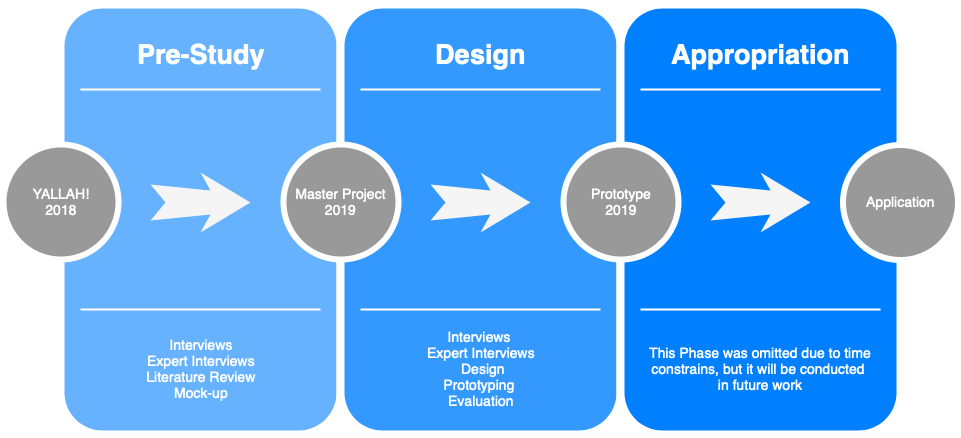
\includegraphics[width=0.90\textwidth]{images/DCS_Diagram.png}
    \caption{Design Case studies Timeline}
    \label{fig:dcs}
\end{figure}
In the Design phase I analyzed the data that I collected in the Pre-study, like practices that people do to be able to see how is the life in Palestine, and what would it be a better experience for the user, I designed the Application upon the results of the data. The Appropriation phase is to analyze the impact of ICT artifact on the transformation towards social practices\citep{Wulf2011}. The researcher will be able to observe the effect of the design on the practice through a certain amount of time. I omitted the Appropriation phase due to time constraints but it will be conducted in further future work with the application.   


\section{Action Research}

Kurt Lewin sometimes called \say{The father of action research}\footnote{The real father of action research is Jacob L. Moreno (1892-1974) who developed the idea in Germany in the 1920s.} described action research in terms of a cycle of steps of planning a change \citep{KemmisSdanMcTaggart1988}.
Action research is a framework that enables the researcher to investigate and evaluate his work \citep{Khanna2007AllResearch}. Also, it is specifically cooperative, interdisciplinary, and interactive. Action research primary focuses on iterative action on the research implementation process for ICT artifacts or any other process, the significant measures are the research results and the viability of the artifact. A spiral cycle that contains planning, acting, observing and reflection, it enables the researcher to take action and observe the results and then to reflect and take action again and so on \citep{Hayes2011TheInteraction}. 
\begin{figure}[ht]
    \centering
    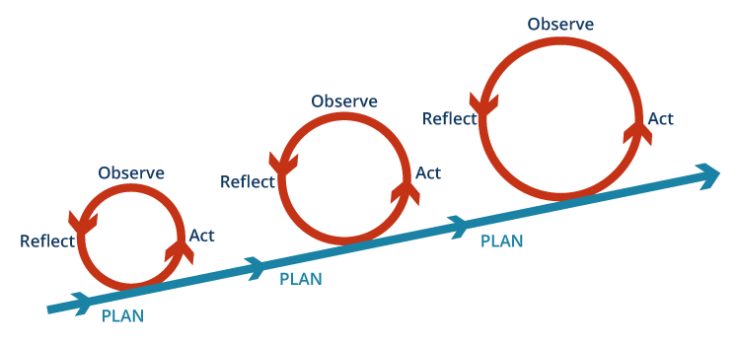
\includegraphics[width=0.90\textwidth]{images/par.png}
    \caption{Action Research steps - © wiobyrne.com  }
    \label{fig:par}
\end{figure}

This \say{spiral of action research} is now familiar to many people. Action research is hardly as smooth as implies this sequence of self-contained loops of planning acting observing and reflecting. The stages intersect, and in the light of learning from experience, initial plans easily become redundant. The process is likely to be faster, more transparent and more adaptive \citep{KemmisSdanMcTaggart1988}. I made several enhancements on the application through the pre-study phase. Action research highlighted the results for me, e.g. \acrfull{ui} it had significant enhancements after I observed the actions and reflected on them, and that implies the whole application as well.     


\section{Qualitative Ethnographic Research Methods}

In the following section, I will define some Ethnographic methods that I conducted through the research. I will also present how I used those methods to gather qualitative data from the field and the user. I conducted several interviews with multidisciplinary people in Germany and Palestine, followed by expert interviews to get a wider view of Virtual Reality from experts. I also took some notes during my trip to Palestine and I will explain it as a method and in the next sections.        

\subsection{Interviews}

“The Interview is a highly used method of collecting data in qualitative social research methods” \citep{Anyan2013}. \cite{Kvale1983} described the purpose of the interview as a method of data collection in social research as “...to gather descriptions of the life-world of the interviewee with respect to interpretation of the meaning of the described phenomena” \cite[p.174]{Kvale1983}. Interviews can provide perspectives and useful data from participants. An important source of insights is by having a conversation with the right participants and interact with them. 
Three types of interviews are unstructured interviews, semi-structured and fully structured interviews \citep{Lazar2017ResearchInteraction}. Unstructured interviews are more like a free-form conversation, without any planned questions or guidelines. A semi-structured interview is using established questions that were planned out, but the interviewer can ask additional follow-up questions as the interviewer see it appropriate and not only commit to the questions guideline. This loose structure and the open-ended interview are benefits for collecting additional insights in the interview \citep{Pannafino2017UXMethods}. A fully structured interview is a more quantitative research method where the interviewer follows the flow of the structured questions in the guideline to obtain data about a specific objective usually employed in survey research. Therefore, direct conversations with participants can provide qualitative data that a survey can miss \citep{Lazar2017ResearchInteraction}. \say{If you don't listen to your users, you might miss some of the most important feedback that you can get} \cite [p.187]{Lazar2017ResearchInteraction}. Although the surveys can validate the findings of the interviews within a large population of \citep{Pannafino2017UXMethods}. During the interview, the interviewer needs to listen carefully and take notes while deciding which comments to pursue. It is better to also record the interview with the participant consent, therefore, the interviewer can refer back to the interview later and use it to analyze the data. Analysis of raw-notes and recorder interviews is a challenge because of deciding which is good data and which is bad, then the interviewer will generate a key of findings depending on the theme or pattern that he followed \citep{Lazar2017ResearchInteraction, Pannafino2017UXMethods}.
I conducted twelve semi-structured and open-ended interviews with multi-disciplinary people in Germany and Palestine, six of the interviews were with privileged second and third Palestinian refugee/immigrant generations living in Germany, two interviews with refugees from Al-Ghabisiyya village and another two interviews with Palestinian refugees in the Westbank. One interview with a high school student from Ramallah, and another interview with a senior man from Jerusalem. Nine of those interviews were recorded and the participants signed a declaration of consent, the rest of the interviews were not recorded due to some technical difficulties but I took notes during all the interviews. Then I transcript all the interviews and analyzed all the data and got major insights that were clear and came from all the participants.           

\subsection{Expert Interview}
The expert interview was designed to explore expert knowledge, it is a qualitative research method. Only the researcher decides whom to conduct an interview with as an expert. Expert Interviews according to \cite{Christmann2016}  “in scientific research an individual is addressed as an expert because the researcher assumes – for whatever reason – that she or he has knowledge, which she or he may not necessarily possess alone, but which is not accessible to anybody in the field of action understudy” \cite[p.18]{Christmann2016}. Although, Experts knowledge must be unique and not accessible by everyone, otherwise it wouldn't be considered as expertise. \say{An expert is someone who is responsible in some way or another for the development, implementation or monitoring of a problem or who has privileged access to information about people or decision processes} \cite[p.221]{Christmann2016}. Conducting the expert interview in purpose to explore a certain phase in a project would be concentrated and efficient for gathering data in a short time. As well it will be easier and faster to obtain good results from the expert interviews. I conducted two informal interviews with experts, hence it was more like an intellectual conversation and I gained data and experience from those interviews, the first interview was with a Virtual Reality expert, and the second one was with an expert in the Palestinian villages and stories about the Palestinian Nakba \say{Catastrophe}. None of these interviews were recorded, but notes were taken by paper and pen. 

\subsection{Field Notes}

Field notes are a necessary part of the ethnographic research. Researchers take notes during observations and conversations in the field, they are defined as a shorthand reconstruction of events. Researchers and ethnographers decide about what they want to write about while they are in the field \citep{Wolfinger2002OnExpectancies}. Those decisions that are taken by researchers and ethnographers are usually unarticulated and invisible to the reader. The field notes would construct the field trip with brief narratives from the moment that the researcher enters the field to the moment he leaves while the field site is not confined in a particular location. The researcher must take notes about every single detail not only through the interview but about the artifacts, the landscape the surrounding circumstances also events on the ground. Not all the data should be always formally documented, researchers and ethnographers should also pay attention to the unrecorded or not captured moments during the fieldwork \citep{Boulus-rdje2018StuckSite}. I took notes while I was conducting interviews, I was writing notes from the participants but I also was writing their reactions, if they were getting excited or emotional. During the field trip, I tried to take as many notes as possible, but I always wrote all the notes by the end of the day when I arrive home.   

\section{Prototyping}

A prototype is an initial representation of a design that is made in a purpose of testing before producing the final artifact \citep{Buchenau2000ExperiencePrototyping}. Prototyping is the core factor for exploring and testing the designs for interactive systems. Prototypes will evaluate the new design and examine it, as well as present the problems in the design \citep{Buchenau2000ExperiencePrototyping, Houde1997WhatPrototype}. Despite which medium the designer is using, a prototype can always represent the design idea. Three dimensions are important for any interactive design, role, look and feel, and implementation. The role is asking about how the artifact is useful for the user's life. Look and feel, questions the experience of the user and what the user sees and feels or hears from the artifact. Implementation refers to the functionality of the artifact and how does it work. The prototype might present design options from one or two or three dimensions of the model \citep{Houde1997WhatPrototype, Buchenau2000ExperiencePrototyping}. I built a prototype that contained a 360$^{\circ}$ video from Damascus gate in Jerusalem. The prototype was a mobile application that I implemented on my smartphone and I used Google daydream \acrshort{vr} glasses to let the users try it. later on, I enhanced the prototype with a better interface. The interface helped the users to see different locations of the city. The prototype gave me good insights from the users and gave the users a better idea about the application.

\section{Thinking Aloud}

Thinking aloud is commonly used in digital platforms for usability testing \citep{VanWaes2000}. The thinking-aloud approach consists of making a user interact with a computer system (prototype, paper mock-up or documentation),  automatically users start expressing thoughts, data, intentions, opinions, hopes, fears, anxieties, etc.  Thinking aloud is a process that provides participants with a model in a situation and is often tested by participants reflecting on how they use the prototype. Each verbalization is transcribed and then analyzed in a formal analysis process. In the context of the informal guidelines, observers are asked to take note of what the participants say and do without attempting to interpret their actions and words, particularly where they encounter difficulties \citep{Jrgensen1990}. There are two kinds of thinking aloud techniques, retrospective think-aloud, and concurrent think aloud. Retrospective think-aloud is a specific situation is recorded or verbalized after the experience. Concurrent think-aloud it is handled while the users are experimenting with a specific task, like solving a problem, surfing the web or navigating a \acrshort{vr} environment \citep{Friedman2004NavigatingSteps}. According to \cite{Marsh1999EvaluationUsability} the main difference between a two-dimensional digital interface and \acrfull{vr} system, that the evaluation happens from inside the \acrshort{vr} environment. Thinking aloud in \acrshort{vr} applications measure the user performance on two levels, the user performance with the \acrshort{vr} application, and the behavior of the user inside the \acrshort{vr} application \citep{Marsh1999EvaluationUsability}. I conducted thinking aloud sessions after each interview with the participants, I
took notes while I was observing the users behavior in the \acrshort{vr} application. By following
a concurrent think-aloud type, users were asking me questions and sometimes I asked
them to do some specific tasks. After the test finish, I asked them for their feedback and
to evaluate the application. 





